\section{Exploratory Data Analysis}

\subsection{Measures of Dispersion}

Data tends to cluster toward the center of the frequency distribution, but extreme values can be far from this central tendency. Measures of dispersion quantify this distance from the average.

\subsubsection{Range}

The difference between the upper and lower limits of a dataset. Limited utility as it is easily affected by extreme values. The interquartile range (IQR) is commonly used to suppress the influence of extremes (Witte y Witte, 2017).

\subsubsection{Quartiles and Interquartile Range}

Quartiles divide the distribution into four equal parts (25\% each). Q1 (25th percentile), Q2 (median, 50th percentile), and Q3 (75th percentile). The IQR equals Q3 - Q1, representing the range for the middle 50\% of data, effectively removing the upper and lower 25\%. The IQR is resistant to extreme values and tends to be less than half the range (Witte y Witte, 2017).

\begin{figure}[H]
\centering
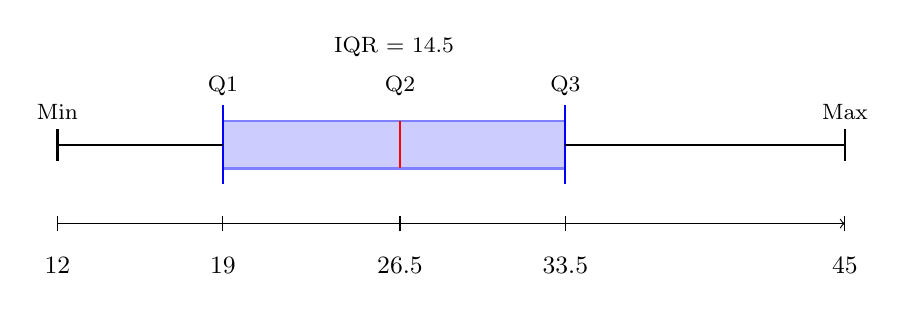
\begin{tikzpicture}[scale=1]
    % Scale: compressed to fit page
    % Values: Min=12, Q1=19, Q2=26.5, Q3=33.5, Max=45
    % Compressed positions: 0, 2.1, 4.35, 6.45, 10
    
    % Draw the number line
    \draw[->] (0,-1) -- (10,-1);
    \foreach \x in {0,2.1,4.35,6.45,10} {
        \draw (\x, -1.1) -- (\x, -0.9);
    }
    \node[below, font=\small] at (0, -1.3) {12};
    \node[below, font=\small] at (2.1, -1.3) {19};
    \node[below, font=\small] at (4.35, -1.3) {26.5};
    \node[below, font=\small] at (6.45, -1.3) {33.5};
    \node[below, font=\small] at (10, -1.3) {45};
    
    % Draw the box (IQR) - from Q1 to Q3
    \draw[fill=blue!20, draw=blue!50, thick] (2.1, -0.3) rectangle (6.45, 0.3);
    
    % Draw median line (Q2)
    \draw[thick, red] (4.35, -0.3) -- (4.35, 0.3);
    
    % Draw quartile markers
    \draw[thick, blue] (2.1, -0.5) -- (2.1, 0.5);
    \draw[thick, blue] (6.45, -0.5) -- (6.45, 0.5);
    
    % Labels
    \node[above, font=\footnotesize] at (2.1, 0.5) {Q1};
    \node[above, font=\footnotesize] at (4.35, 0.5) {Q2};
    \node[above, font=\footnotesize] at (6.45, 0.5) {Q3};
    \node[above, font=\footnotesize] at (4.275, 1) {IQR = 14.5};
    
    % Whiskers (from min to Q1 and Q3 to max)
    \draw[thick] (0, 0) -- (2.1, 0);
    \draw[thick] (6.45, 0) -- (10, 0);
    
    % Min and Max markers
    \draw[thick] (0, -0.2) -- (0, 0.2);
    \draw[thick] (10, -0.2) -- (10, 0.2);
    \node[above, font=\footnotesize] at (0, 0.2) {Min};
    \node[above, font=\footnotesize] at (10, 0.2) {Max};
\end{tikzpicture}
\caption{Box plot showing quartiles and interquartile range. The box represents the IQR (middle 50\% of data), Q1 and Q3 are the box edges, and Q2 (median) is the red line.}
\label{fig:quartiles_example}
\end{figure}

\subsubsection{Variance}

The average of the squared deviations from the arithmetic mean. Deviations are squared because their sum equals zero (negative cancel positive). Notation: $s^2$ (sample) and $\sigma^2$ (population). Useful for comparing variability between distributions, but has squared units making interpretation complex (Spiegel y Stephen, 2009).

The formulas for variance are:

\begin{align}
\text{Population variance: } \sigma^2 &= \frac{1}{N}\sum_{i=1}^{N}(x_i - \mu)^2 \\
\text{Sample variance: } s^2 &= \frac{1}{n-1}\sum_{i=1}^{n}(x_i - \bar{x})^2
\end{align}

where $N$ is the population size, $n$ is the sample size, $\mu$ is the population mean, and $\bar{x}$ is the sample mean.

\paragraph{Example: Calculating Variance}

Consider the following dataset representing test scores: 75, 82, 68, 90, 85.

\textit{Note: This example calculates sample variance ($s^2$), treating the data as a sample from a larger population. If this were the entire population, we would use population variance ($\sigma^2$) and divide by $N$ instead of $(n-1)$.}

\textbf{Step 1: Calculate the mean}
\begin{equation}
\bar{x} = \frac{75 + 82 + 68 + 90 + 85}{5} = \frac{400}{5} = 80
\end{equation}

\textbf{Step 2: Calculate deviations from the mean}
\begin{align}
x_1 - \bar{x} &= 75 - 80 = -5 \\
x_2 - \bar{x} &= 82 - 80 = 2 \\
x_3 - \bar{x} &= 68 - 80 = -12 \\
x_4 - \bar{x} &= 90 - 80 = 10 \\
x_5 - \bar{x} &= 85 - 80 = 5
\end{align}

\textbf{Step 3: Square each deviation}
\begin{align}
(x_1 - \bar{x})^2 &= (-5)^2 = 25 \\
(x_2 - \bar{x})^2 &= (2)^2 = 4 \\
(x_3 - \bar{x})^2 &= (-12)^2 = 144 \\
(x_4 - \bar{x})^2 &= (10)^2 = 100 \\
(x_5 - \bar{x})^2 &= (5)^2 = 25
\end{align}

\textbf{Step 4: Sum the squared deviations}
\begin{equation}
\sum_{i=1}^{5}(x_i - \bar{x})^2 = 25 + 4 + 144 + 100 + 25 = 298
\end{equation}

\textbf{Step 5: Calculate sample variance}
\begin{equation}
s^2 = \frac{1}{n-1}\sum_{i=1}^{n}(x_i - \bar{x})^2 = \frac{1}{5-1} \times 298 = \frac{298}{4} = 74.5
\end{equation}

Therefore, the sample variance is $s^2 = 74.5$ (units squared).

\subsubsection{Standard Deviation}

To resolve the problem of squared units of measurement, the square root of the variance is calculated, always taking the positive value. This produces a new measure, known as standard deviation, which describes variability in the original units of measurement. Like the previous measures, standard deviation must be distinguished: symbolized by $s$ for the sample and $\sigma$ for the population.

The formulas for standard deviation are:

\begin{align}
\text{Population standard deviation: } \sigma &= \sqrt{\sigma^2} = \sqrt{\frac{1}{N}\sum_{i=1}^{N}(x_i - \mu)^2} \\
\text{Sample standard deviation: } s &= \sqrt{s^2} = \sqrt{\frac{1}{n-1}\sum_{i=1}^{n}(x_i - \bar{x})^2}
\end{align}

\paragraph{Example: Calculating Standard Deviation}

Using the previous variance example (test scores: 75, 82, 68, 90, 85), where we calculated $s^2 = 74.5$:

\begin{equation}
s = \sqrt{s^2} = \sqrt{74.5} \approx 8.63
\end{equation}

Therefore, the sample standard deviation is $s \approx 8.63$ test score points.

\paragraph{Interpretation}

The standard deviation measures the typical distance of data points from the mean. In this example:
\begin{itemize}
    \item The mean test score is 80 points
    \item The standard deviation is approximately 8.63 points
    \item This means that, on average, test scores deviate from the mean by about 8.63 points
    \item Most scores (approximately 68\% in a normal distribution) fall within one standard deviation of the mean, i.e., between $80 - 8.63 = 71.37$ and $80 + 8.63 = 88.63$ points
\end{itemize}

\begin{tcolorbox}[colback=blue!5!white, colframe=blue!75!black, title=Curious Fact]
A larger standard deviation indicates greater variability (scores are more spread out), while a smaller standard deviation indicates less variability (scores are clustered closer to the mean).
\end{tcolorbox}

\subsection{Outlier Detection}

An outlier is a numerical observation that is distant from the rest of the data. Outliers in a dataset can cause problems in statistical analyses by generating misleading conclusions. Usually, an outlier can indicate a measurement error or a long-tailed distribution in the population, although they can occur by chance.

\subsubsection{Box Plot}

A box plot is a graphical representation of numerical data through its quartiles. The boxes in this standardized method contain the following elements: the median (Q2), the interquartile range, and the quartiles (Q1 and Q3). Box plots also have lines extending from the boxes (whiskers) that indicate variability outside the upper and lower quartiles, hence the term box-and-whisker plot. Depending on the type of representation, the whiskers can extend to the minimum value at one end and the maximum value at the other, representing the full range.

For outlier identification, John Tukey proposed whiskers with a length of 1.5 times the IQR (Tukey, 1977). That is, from the hinges (Q1 and Q3), 1.5 times the IQR is added or subtracted respectively. Then, values beyond these whiskers are considered outliers and are represented as individual points.

To construct box plots, the median, first and third quartiles, and the interquartile range of each attribute are used. Then, for the whiskers, 1.5 times the IQR is added above and subtracted below the box. Finally, the last value within those limits is taken, and that is where the whiskers are graphed.

\paragraph{Example: Box Plot with Outliers}

Consider the dataset: 10, 12, 14, 16, 18, 20, 22, 24, 26, 28, 30, 32, 60, 70.

Calculating the quartiles:
\begin{itemize}
    \item Q1 = 16, Q2 (median) = 23, Q3 = 30
    \item IQR = Q3 - Q1 = 30 - 16 = 14
    \item Lower whisker limit: Q1 - 1.5 × IQR = 16 - 21 = -5 (minimum within limit: 10)
    \item Upper whisker limit: Q3 + 1.5 × IQR = 30 + 21 = 51
    \item Outliers: 60 and 70 (both exceed the upper whisker limit)
\end{itemize}

\textit{Note: The whiskers extend to 10 and 32, not to the calculated limits (-5 and 51). This is because whiskers are drawn to the last data value within the limits, not to the limits themselves. Since -5 is below any actual data point, the lower whisker goes to the minimum value (10). Similarly, the upper whisker stops at 32, which is the last value within the upper limit (51). Values beyond these limits (60 and 70) are shown as outlier points.}

Figure~\ref{fig:boxplot_outliers} shows the box plot for this dataset, with outliers represented as individual points.

\begin{figure}[H]
\centering
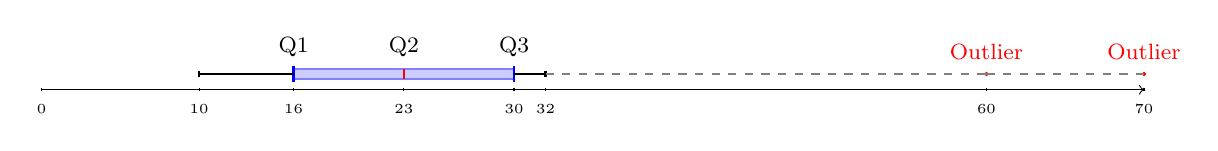
\begin{tikzpicture}[scale=0.2]
    % Values: Q1=16, Q2=23, Q3=30, IQR=14
    % Lower whisker: 10, Upper whisker: 51 (but max within limit is 32)
    % Outliers: 60, 70
    
    % Draw the number line
    \draw[->] (0,-1) -- (70,-1);
    \foreach \x in {0,10,16,23,30,32,60,70} {
        \draw (\x, -1.1) -- (\x, -0.9);
    }
    \node[below, font=\tiny] at (0, -1.3) {0};
    \node[below, font=\tiny] at (10, -1.3) {10};
    \node[below, font=\tiny] at (16, -1.3) {16};
    \node[below, font=\tiny] at (23, -1.3) {23};
    \node[below, font=\tiny] at (30, -1.3) {30};
    \node[below, font=\tiny] at (32, -1.3) {32};
    \node[below, font=\tiny] at (60, -1.3) {60};
    \node[below, font=\tiny] at (70, -1.3) {70};
    
    % Draw the box (IQR) - from Q1 to Q3
    \draw[fill=blue!20, draw=blue!50, thick] (16, -0.3) rectangle (30, 0.3);
    
    % Draw median line (Q2)
    \draw[thick, red] (23, -0.3) -- (23, 0.3);
    
    % Draw quartile markers
    \draw[thick, blue] (16, -0.5) -- (16, 0.5);
    \draw[thick, blue] (30, -0.5) -- (30, 0.5);
    
    % Labels
    \node[above, font=\footnotesize] at (16, 0.5) {Q1};
    \node[above, font=\footnotesize] at (23, 0.5) {Q2};
    \node[above, font=\footnotesize] at (30, 0.5) {Q3};
    
    % Whiskers (from Q1 to lower limit and Q3 to upper limit within bounds)
    \draw[thick] (10, 0) -- (16, 0);
    \draw[thick] (30, 0) -- (32, 0);
    
    % Whisker markers
    \draw[thick] (10, -0.2) -- (10, 0.2);
    \draw[thick] (32, -0.2) -- (32, 0.2);
    
    % Outliers as individual points
    \filldraw[red] (60, 0) circle (3pt);
    \filldraw[red] (70, 0) circle (3pt);
    \node[above, font=\footnotesize, red] at (60, 0.3) {Outlier};
    \node[above, font=\footnotesize, red] at (70, 0.3) {Outlier};
    
    % Draw lines from box to outliers (dashed)
    \draw[dashed, gray, thin] (32, 0) -- (60, 0);
    \draw[dashed, gray, thin] (60, 0) -- (70, 0);
\end{tikzpicture}
\caption{Box plot showing quartiles, IQR, whiskers (extending 1.5 × IQR from Q1 and Q3), and outliers (60 and 70) represented as individual red points.}
\label{fig:boxplot_outliers}
\end{figure}

\subsection{Scatter Plots}

The most useful graphical representations for describing the behavior of a set of variables are scatter plots, also known as dot plots or scatter diagrams. These graphs show the relationship between numerical variables, and they allow discovering and confirming anticipated relationships between two associated sets of data. Numerical variables are represented by coordinates in n-dimensional Euclidean space.

\subsubsection{Two-dimensional Scatter Plots}

For the case of two variables, the datasets must have the same length: one for the X-axis (horizontal) and one for the Y-axis (vertical). In Python, a scatter plot of two numerical variables X and Y can be obtained using the \texttt{plot(X, Y)} command from the matplotlib library.

The representation of each variable on each axis allows identifying the relationship of increase or decrease between the dependent and independent variables. Scatter plots are suitable when you have paired numerical data and want to see if one variable affects another. However, it is necessary to understand that correlation is not causation, and another unnoticed variable may influence the results. In the case of a database, numerical variables correspond to dataset attributes and are used to define aspects of an instance, such as size, shape, and color.

\paragraph{Correlation vs. Causation}

\textbf{Example:} Consider a scatter plot showing ice cream sales (X-axis) and drowning deaths (Y-axis) over time. The plot would likely show a positive correlation: as ice cream sales increase, drowning deaths also increase. However, this does not mean that ice cream sales \textit{cause} drowning deaths.

\textbf{Why correlation is not causation:} Both variables are influenced by a third, hidden variable: the season (summer). In summer:
\begin{itemize}
    \item More people buy ice cream (hot weather)
    \item More people go swimming (hot weather)
    \item More swimming leads to more drowning incidents
\end{itemize}

The correlation exists because both variables respond to the same underlying factor (summer weather), not because one directly causes the other. This illustrates that:
\begin{itemize}
    \item \textbf{Correlation} means two variables tend to change together
    \item \textbf{Causation} means one variable directly causes changes in another
    \item A correlation can exist without causation when a third variable (confounding variable) influences both
\end{itemize}

To establish causation, controlled experiments or additional evidence are needed, not just observational correlation.

\paragraph{Example: Scatter Plot}

Figure~\ref{fig:scatter_plot} shows an example of a two-dimensional scatter plot displaying the relationship between two variables. Each point represents a pair of values (x, y), allowing visualization of patterns, trends, and potential correlations in the data.

\begin{figure}[H]
\centering
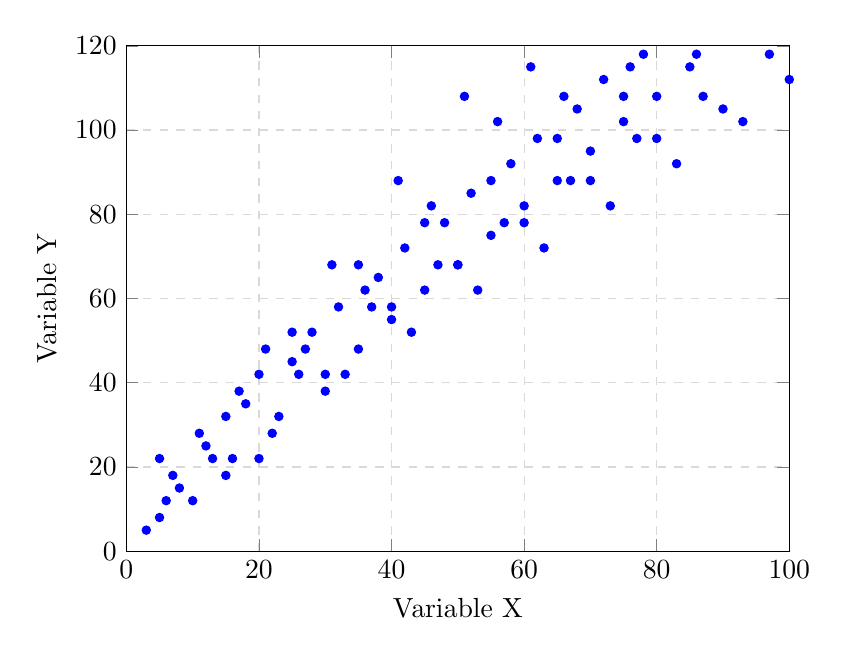
\begin{tikzpicture}
\begin{axis}[
    width=10cm,
    height=8cm,
    xlabel={Variable X},
    ylabel={Variable Y},
    xmin=0,
    xmax=100,
    ymin=0,
    ymax=120,
    grid=major,
    grid style={dashed, gray!30},
]
\addplot[
    only marks,
    mark=*,
    mark size=1.5pt,
    color=blue,
] coordinates {
    (5, 8) (8, 15) (12, 25) (15, 18) (18, 35) (20, 42) (22, 28) (25, 45) (28, 52) (30, 38)
    (32, 58) (35, 48) (38, 65) (40, 55) (42, 72) (45, 62) (48, 78) (50, 68) (52, 85) (55, 75)
    (58, 92) (60, 82) (62, 98) (65, 88) (68, 105) (70, 95) (72, 112) (75, 102) (78, 118) (80, 108)
    (5, 22) (10, 12) (15, 32) (20, 22) (25, 52) (30, 42) (35, 68) (40, 58) (45, 78) (50, 68)
    (55, 88) (60, 78) (65, 98) (70, 88) (75, 108) (80, 98) (85, 115) (90, 105) (95, 122) (100, 112)
    (3, 5) (7, 18) (13, 22) (17, 38) (23, 32) (27, 48) (33, 42) (37, 58) (43, 52) (47, 68)
    (53, 62) (57, 78) (63, 72) (67, 88) (73, 82) (77, 98) (83, 92) (87, 108) (93, 102) (97, 118)
    (6, 12) (11, 28) (16, 22) (21, 48) (26, 42) (31, 68) (36, 62) (41, 88) (46, 82) (51, 108)
    (56, 102) (61, 115) (66, 108) (71, 122) (76, 115) (81, 125) (86, 118) (91, 128) (96, 122) (99, 130)
};
\end{axis}
\end{tikzpicture}
\caption{Example of a two-dimensional scatter plot showing a positive correlation between Variable X and Variable Y.}
\label{fig:scatter_plot}
\end{figure}

\subsubsection{Scatter Plot Matrix}

The scatter plot matrix (SPLOM---scatterplot matrix) presents multiple adjacent scatter plots for all variable comparisons in a single display. To some extent, it addresses one of the geometric problems for datasets with more than three attributes by presenting two or more pairs of variables in the same graph, which is very useful for identifying dependencies between data.

One of the disadvantages is that SPLOM requires a large amount of screen space, and the formation of multivariate associations remains a challenge. Additionally, it is necessary to incorporate additional statistical measures to organize SPLOM and guide the observer through an exploratory analysis of high-dimensional datasets.

\subsection{Correlation between Variables}

\subsubsection{Linear Correlation}

Correlation is known as a statistical measure that quantifies the degree of joint variation that exists between two variables and, specifically, evaluates the increasing or decreasing trend of the data. The types of correlation can be observed in Table~\ref{tab:correlation_types}.

\begin{table}[H]
\centering
\begin{tabular}{|p{5cm}|p{10cm}|}
\hline
\textbf{Type of Correlation} & \textbf{Description} \\
\hline
\textbf{Positive correlation} & The values of the variables increase together, given that an increase in Y (dependent variable) depends on an increase in X (independent variable). \\
\hline
\textbf{Negative correlation} & One value decreases as the other increases; therefore, an increase in the values of variable X will cause a decrease in the values of variable Y. \\
\hline
\textbf{Null or no correlation} & There is no relationship between the variables, therefore, the variables are independent. The graph does not follow any trend, causing the points to be totally dispersed. \\
\hline
\textbf{Linear} & There is a relationship between the variables, which is linear. \\
\hline
\textbf{Non-linear} & Although there is a relationship between the variables, it is not linear. It can be exponential, U-shaped, etc. \\
\hline
\end{tabular}
\caption{Types of correlation}
\label{tab:correlation_types}
\end{table}

Given the subjectivity in interpreting scatter plots, it is necessary to use a coefficient that allows measuring the degree of dependence between variables. The linear correlation coefficient represents the behavior of a dependent variable Y with respect to an independent variable X.

The strength of the correlation is determined by the proximity of the points to each other in the graph. If the points are closer together, the strength will be greater (strong correlation). If they are not so concentrated, the strength will be weak. If a pattern of very dispersed points is observed, the correlation strength will be null (no correlation).

\subsubsection{Pearson's Correlation Coefficient}

Pearson's correlation coefficient is a statistic whose values range between -1 and 1 ($-1 \leq r \leq 1$). A correlation close to 1 indicates a positive association (both variables increase together). A correlation close to -1 indicates a negative association (one increases as the other decreases). A value near 0 indicates no linear relationship, although a non-linear relationship may exist. This coefficient can only be used for quantitative and continuous variables.

The correlation coefficient is calculated as:

\begin{equation}
r = \frac{\text{Cov}(X,Y)}{S_x \cdot S_y}
\end{equation}

where:
\begin{itemize}
    \item $r$ is Pearson's correlation coefficient
    \item $\text{Cov}(X,Y)$ is the covariance between X and Y
    \item $S_x$ is the standard deviation of variable X
    \item $S_y$ is the standard deviation of variable Y
\end{itemize}

This coefficient allows determining the existence and intensity of linear associations between variables. The sign is interpreted the same as covariance: positive (direct correlation), negative (inverse correlation), or null (no correlation). It measures how close the points are to a straight line, reflecting the data trend.

\begin{tcolorbox}[colback=blue!5!white, colframe=blue!75!black, title=Curious Fact: Covariance]
Covariance measures how two variables vary together. It is calculated as the average of the products of deviations from the mean: $\text{Cov}(X,Y) = \frac{1}{n-1}\sum(x_i - \bar{x})(y_i - \bar{y})$. A positive covariance means that when X is above its mean, Y tends to be above its mean too (they move together). A negative covariance means when X is above its mean, Y tends to be below its mean (they move in opposite directions). However, covariance is difficult to interpret because its magnitude depends on the units of measurement. This is why Pearson's correlation coefficient normalizes covariance by dividing by the product of standard deviations, making it unitless and easier to interpret.
\end{tcolorbox}

\paragraph{Example: Calculating Pearson's Correlation Coefficient}

Consider the following paired dataset:
\begin{center}
\begin{tabular}{c|c}
X & Y \\
\hline
2 & 4 \\
4 & 6 \\
6 & 8 \\
8 & 10 \\
10 & 12 \\
\end{tabular}
\end{center}

\textbf{Step 1: Calculate the means}
\begin{align}
\bar{x} &= \frac{2 + 4 + 6 + 8 + 10}{5} = \frac{30}{5} = 6 \\
\bar{y} &= \frac{4 + 6 + 8 + 10 + 12}{5} = \frac{40}{5} = 8
\end{align}

\textbf{Step 2: Calculate deviations and their products}
\begin{align}
\sum (x_i - \bar{x})(y_i - \bar{y}) &= (2-6)(4-8) + (4-6)(6-8) + (6-6)(8-8) + (8-6)(10-8) ...\\
&= (-4)(-4) + (-2)(-2) + (0)(0) + (2)(2) + (4)(4) \\
&= 16 + 4 + 0 + 4 + 16 = 40
\end{align}

\textbf{Step 3: Calculate standard deviations}
\begin{align}
S_x &= \sqrt{\frac{1}{n-1}\sum(x_i - \bar{x})^2} = \sqrt{\frac{(-4)^2 + (-2)^2 + 0^2 + 2^2 + 4^2}{4}} = \sqrt{\frac{40}{4}} = \sqrt{10} \approx 3.16 \\
S_y &= \sqrt{\frac{1}{n-1}\sum(y_i - \bar{y})^2} = \sqrt{\frac{(-4)^2 + (-2)^2 + 0^2 + 2^2 + 4^2}{4}} = \sqrt{\frac{40}{4}} = \sqrt{10} \approx 3.16
\end{align}

\textbf{Step 4: Calculate covariance}
\begin{equation}
\text{Cov}(X,Y) = \frac{1}{n-1}\sum(x_i - \bar{x})(y_i - \bar{y}) = \frac{40}{4} = 10
\end{equation}

\textbf{Step 5: Calculate Pearson's correlation coefficient}
\begin{equation}
r = \frac{\text{Cov}(X,Y)}{S_x \cdot S_y} = \frac{10}{3.16 \times 3.16} = \frac{10}{10} = 1.0
\end{equation}

Therefore, $r = 1.0$, indicating a perfect positive linear correlation. This makes sense as the data points lie exactly on a straight line with a positive slope.

\subsection{Covariance Matrix}

Statistics allow understanding relationships between multiple variables simultaneously. If covariance is positive, the linear association is positive. If covariance is negative, the linear association is negative (small X values correspond to large Y values, and vice versa).

The covariance matrix is a square matrix containing variances on the main diagonal and covariances in the off-diagonal elements. The matrix is symmetric: the covariance between X and Y equals the covariance between Y and X, so each pair appears twice.
